\section{Øvelse 9 - UDP/IP socket programming}

\subsection{Introduktion}
I denne øvelse i socket programmering, udarbejdes en UDP client og en UDP server. Igen er C\# valgt som programmeringssprog. Clienten forbinder til serveren og downloader en fil herfra. Clienten o server køres på hver sin virtuelle linux maskine. I dette dokument beskrives udviklingsforløbet med tilhørende diagrammer og kodeforklaringer.

\subsection{Udviklingsforløb}
Der oprettes først en forbindelse mellem server og client. Derefter sender clienten en request til serveren, hvorefter denne checker om der findes en matchende kommande til clientens request.
Såfremt serveren finder en matchende kommando, aflæses den rette server status, som derefter sendes tilbage til clienten.

\begin{lstlisting}[caption = Hoveddesign for server,label=code:udpServer]
private static void StartListener() 
{
	//Initiate UDP server
	
	while(true) 
	{
		//Wait for incoming command
		//Send matching response
	}
}
\end{lstlisting}

\begin{lstlisting}[caption = Hoveddesign for client,label=code:udpClient]
static void Main(string[] args)
{
	//Setup UDP client
	//Initialize ip and command from args
	//Send command
	//Wait for answer and output to console
}
\end{lstlisting}

\subsection{Funktionalitet}
Herunder beskrives virkemåde for koden som er skrevet udfra psudokoden i vist i \ref{code:udpServer}. Yderligere kan et sekvensdiagram for UDP koden ses på figur \ref{fig:sequence2} på side \pageref{fig:sequence2}.

\begin{enumerate}
	\item Først initializeres en UDP server og en socket.
	\item Serveren venter derefter på at modtage en kommando fra en klient. Der skrives i konsollen hvilken
	kommando som er modtaget, samt hvem afsenderen var.
	\item Der tjekkes på den modtagne kommando, og sendes et matchende svar. Desuden skrives i konsollen
	hvilken kommando der bliver sendt, samt indholdet af kommandoen.
\end{enumerate}

Her beskrives virkemåden for koden i codeudsnit \ref{code:udpClient} for klienten.

\begin{enumerate}
	\item Først initializeres der en UDP client og en socket.
	\item Der indlæses ip adresse og kommando fra brugerens argumenter.
	\item Kommandoen sendes til serveren.
	\item Der ventes på at serveren svarer, og det modtagne svar udskrives i konsollen.
\end{enumerate}

\subsection{Resultater}
Vi har testet vores system og vedlagt screenshots heraf. På figur \ref{fig:udp_h1} ses test af serveren. Figur \ref{fig:udp_h2} viser klientens side af udvekslingen. Billederne illusterer desuden programflowet med konsoludskrifter.

\begin{figure}[H]
	\centering
	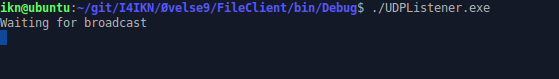
\includegraphics[width=0.9\linewidth]{figs/udp_h1}
	\caption{Test af UDP server/client - billede fra server.}
	\label{fig:udp_h1}
\end{figure}

\begin{figure}[H]
	\centering
	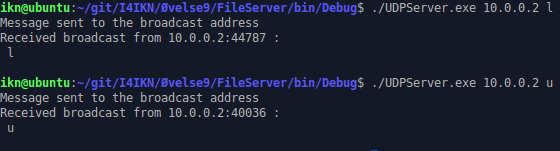
\includegraphics[width=0.9\linewidth]{figs/udp_h2}
	\caption{Test af UDP server/client - billede fra client.}
	\label{fig:udp_h2}
\end{figure}

\subsection{Konklusion}
I arbejdet med UDP socket programmering er vi kommet frem til en løsning der opfylder kravene givet i opgaven. Det kan derfor konstateres at teorien stemmer overens med praksis.